\documentclass[5pt]{article}
\usepackage{multicol,multirow}
\usepackage{graphicx} % Required for inserting images
\usepackage[margin=0.75cm]{geometry}
\usepackage{xcolor}
\usepackage{amsmath,esint}
\usepackage{mathtools}
\usepackage{relsize}
\usepackage{mathtools}
\usepackage{nccmath}
\usepackage[inline]{enumitem}
\usepackage{algpseudocode}

\usepackage{empheq}
\usepackage{amsfonts}

\usepackage{tkz-euclide}
\usepackage{tikz}

\definecolor{LightGray}{gray}{0.9}

\usepackage{minted}

\newenvironment{amatrix}[1]{%
  \left[\begin{array}{@{}*{#1}{c}|c@{}}
}{%
  \end{array}\right]
}

\DeclarePairedDelimiter\abs{\lvert}{\rvert}%
\DeclarePairedDelimiter\norm{\lVert}{\rVert}%

\makeatletter
\let\oldabs\abs
\def\abs{\@ifstar{\oldabs}{\oldabs*}}

\newcommand{\tr}[3]{
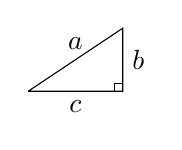
\begin{tikzpicture}[scale=0.40]
    \coordinate [] (A) at (-1.5cm,-1.cm);
    \coordinate [] (C) at (1.5cm,-1.0cm);
    \coordinate [] (B) at (1.5cm,1.0cm);
    \draw (A) -- node[above] {$a$} (B) -- node[right] {$b$} (C) -- node[below] {$c$} (A);
    \draw (1.25cm,-1.0cm) rectangle (1.5cm,-0.75cm);
\end{tikzpicture}
}


\begin{document}


\begin{center}
     \Large{\textbf{Linear Algebra from Elementary to Advanced}}\\
     \footnotesize{University: Johns Hopkins University}\hfill\footnotesize{\textcopyright Maximilien Notz \the\year{}}
     \noindent\rule{20.2cm}{0.4pt}
\end{center}


\begin{multicols}{2}
\setcounter{secnumdepth}{0}


\subsection{Definition}
\begin{tabular}{ll}
    Linear Functions & All terms are of  degree 0 or 1. \\
                   & A solution of a system of linear \\ 
                   & equation is set of points that makes \\
                   & the equation system true. \\
     Consistent    & lin. systems is consistent if either 1 or $\infty$ \\
                   & solutions exist else inconsistent.\\
     Conist
\end{tabular}

\section{Linear Systems and Matrix Equations}
\subsection{Coefficient Matrix Example}
\begin{equation}
\centering
\left\{\begin{split}
A_1x_1+A_2x_2+A_3x_3=\alpha \\
B_1x_1+B_2x_2+B_3x_3=\beta \\
\end{split}\right.
\Leftrightarrow
\begin{bmatrix}
    A_1 & A_2 & A_3\\
    B_1 & B_2 & B_3\\
\end{bmatrix}
\end{equation}

\subsection{Augmented Matrix Example}
\begin{equation}
\left\{\begin{split}
A_1x_1+A_2x_2+A_3x_3=\alpha \\
B_1x_1+B_2x_2+B_3x_3=\beta \\
\end{split}\right.
\Leftrightarrow
\begin{amatrix}{3}
    A_1 & A_2 & A_3 & \alpha \\
    B_1 & B_2 & B_3 & \beta \\
 \end{amatrix}
\end{equation}


\subsection{Row-Equivalence}
Two matrce are row-equivalent if there is a sequence of \textbf{EROS} that transforms one into the other.


\subsection{Elementary Row Operations (EROS)}
1. \textbf{[Replacement]} Replace one row by sum of itself. \\
2. \textbf{[Interchange]} Swap position of 2 rows. \\
3. \textbf{[Scaling]} Multiply all entries in row by non-zero constant. \\


\subsection{Echelon Form (ef)}
1. All non-zero rows are above any rows of all-zero. \\
2. Each leading entry of a row is in a column to the right of the roe above it. \\
3. All entries in a column below a leading entry are 0. \\


\subsection{Reduced Row Echelon Form (rref)}
1. As to be in echelon form. \\
2. Leading entry in each row is 1. \\
3. Each leading 1 is the only non-zero entry in its column. \\


\subsection{Theorems}
\newtheorem{theorem}{Theorem}
\newtheorem{properties}{Properties}
\begin{theorem}
Every matrix is row equivalent to a unique row echelon form.
\end{theorem}

\begin{theorem}
Every matrix is row equivalent to a unique row echelon form.
\end{theorem}

\section{Matrix Algebra, Determinants, \& Eigenvectors}

\section{Orthogonality and Diagonalization}
\subsection{Definition}
\begin{tabular}{ll}
  Inner Product       & $\vec{v}\cdot\vec{u}=\vec{v}^T\vec{u}=u_1v_1 + ... + u_nv_n$\\
                      & \footnotesize{(Also called dot product or scalar product)}\\
  Length of $\vec{x}$ & $||\vec{x}||=\sqrt{\vec{x}\cdot\vec{x}}=\sqrt{x^2_1+...+x^2_n}$\\
                      & \footnotesize{(Also called Norm or Magnitude)}\\
  Unit vectore        & A vector with $||\vec{x}||=1$ \\
  Normalization       & The formula $\vec{u}=\frac{\vec{x}}{||\vec{x}||}$ creat a unit vector \\
                      & in the same direction as $\vec{x}$. \\
  Distance            &  $dist(\color{blue}\vec{u}\color{black},\color{red}\vec{v}\color{black})=\color{blue}\vec{u}\color{black}-\color{red}\vec{v}$      
                        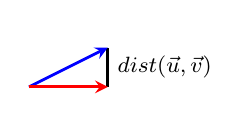
\begin{tikzpicture}[scale=0.50,baseline={([yshift={-\ht\strutbox-12}]current bounding box.north)}]
                          \draw[line width=1pt,black](2,0)--(2,1) node[anchor=south west]{};
                          \draw[line width=1pt,blue,-stealth](0,0)--(2,1) node[anchor=south west]{};
                          \draw[line width=1pt,red,-stealth](0,0)--(2,0) node[anchor=south]{}; 
                          \draw [line width=0.5pt]
                            (2,0.5) coordinate (d) node[right] {\footnotesize$dist(\vec{u},\vec{v})$}
                            (2,0) coordinate (v) node[right] {}
                            (2,1) coordinate (u) node[right] {};
                        \end{tikzpicture}\\
Orthogonality         & $\vec{u}\cdot \vec{v} = 0$
                      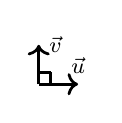
\begin{tikzpicture}[scale=0.5,baseline={([yshift={-\ht\strutbox-10}]current bounding box.north)}]
                        \draw[black,step=0.3, line width=1pt] (0,0) grid (0.3,0.3);
                        \draw[->,line width=1pt] (0,0)--(1,0) node[above]{\footnotesize$\vec{u}$};
                        \draw[->,line width=1pt,] (0,0)--(0,1) node[right]{\footnotesize$\vec{v}$};
                      \end{tikzpicture}\\
Orthogonal Set        & A set  of vectors $\{\vec{u}_1, ..., \vec{u}_p\}\in\mathbb{R}^n$ such that\\ 
                      & each distinct vectors are orthogonal.\\
Orthogonal Basis      & For a subspace $W$ of $R^n$ is a basis that is\\
                      & also an orthogonal set.\\
Orthonormal set       & is a set  of  orthogonal unit vectors.\\
Orthogonal matrix     & Is a squared matrix whose columns are\\
                      & orthonormal.\\
Normal equation       & $A^TA\vec{x}=A^T\vec{b}$\\
least-squares error   & $||\vec{b}-A\hat{x}||$
\end{tabular}
\begin{tabular}{ll}
Orthogonal Complements  & Let $W$ be a subspace of $\mathbb{R}^n$.\\
                        & The orthogonal complement of $W$ is: \\
                        & $W^\perp=\{\vec{x}\in\mathbb{R}^n|\vec{x}\cdot\vec{w}=\vec{0}, \forall\vec{w}\in W\}$\\
Orthogonal Projection   & of $\vec{y}\in\mathbb{R}^n$ onto subspace $W$ of $\mathbb{R}^n$ is\\
                        & the vector $\hat{y}$ in $W$ such that $\vec{y} -\hat{y}$ \\
                        & is in $W^\perp$. (Noted $\text{proj}_W(\vec{y})$)\\
Least-Squares Problem   & is to find $\vec{x}$ that makes $||\vec{b}-A\vec{x}||$ \\
                        & $=\text{dist}(\vec{b},A\vec{x})$ as small as possible.                  
\end{tabular}

\subsection{Theorems}
\begin{properties}
  Let $\vec{u},\vec{v},\vec{w} \in \mathbb{R}^n$ and $c\in \mathbb{R}^n$ then:\\
  \begin{itemize*}
    \item $\vec{u}\cdot\vec{v}=\vec{v}\cdot\vec{u}$ 
    \item $(\vec{u}+\vec{v})\cdot \vec{w}=\vec{u}\cdot\vec{w}+\vec{v}\cdot \vec{w}$
    \item $(c\vec{u})\cdot \vec{v}=c(\vec{u}\cdot \vec{v})=(c\vec{v})\cdot \vec{u}$
    \item $\vec{u}\cdot \vec{u}=u_1^2+...+u^2_n\geq 0$
  \end{itemize*}
\end{properties}

\begin{theorem}[Fundamental Subspaces Theorem]
  Let $A_{M\times N}$ then:
  \begin{itemize*}
    \item $(row(A))^\perp=nul(A)$
    \item $(COl(A))^\perp=nul(a^\perp)$
  \end{itemize*}
\end{theorem}

\begin{theorem}
  If $S=\{\vec{u}_1,...,\vec{u}_p\}$ is an \textbf{orthogonal set} of non-zero vectors in $\mathbb{R}$ then $S$ is a \textbf{linearly independant} set. 
\end{theorem}

\begin{theorem}
  let $\{\vec{u}_1,...,\vec{u}_p\}$ be an \textbf{orthogonal basis} for $w\subset \mathbb{R}^n$. 
  Let $y\in W$. Then $\vec{y}=C_1\vec{u}_1 + ... + C_p\vec{u}_p$, $C_j=\frac{\vec{y}\cdot\vec{u}_i}{\vec{u}_i\cdot\vec{u}_i}$
\end{theorem}

\begin{theorem}
  Let $u=(\vec{u}_1 \vec{u}_2 \vec{u}_3)$, where $\{\vec{u}_1, \vec{u}_2, \vec{u}_3\}$ is orthonormal set.
  $u^T\cdot u= I$
\end{theorem}

\begin{theorem}
  Let $u$ be an \textbf{orthogonal matrix}, Let $\vec{x},\vec{y}\in\mathbb{R}$:
  \begin{itemize*}
    \item $|u\vec{x}|=|\vec{x}|\:$
    \item $(u\vec{x})\cdot(u\vec{y})=\vec{x}\cdot\vec{y}$
  \end{itemize*}
\end{theorem}

\begin{theorem}[Orthogonal Decomposition Theorem]
  Let $W$ be a subspace with an orthogonal basis $\{\vec{u}_1,...,\vec{u}_p\}$. let $\vec{y}\in\mathbb{R}^n$ then: 
  $\hat{y}=\left(\frac{\vec{y}\cdot\vec{u}_1}{\vec{u}_1\cdot\vec{u}_1}\right)\vec{u}_1 + ... + \left(\frac{\vec{y}\cdot\vec{u}_p}{\vec{u}_p\cdot\vec{u}_p}\right)\vec{u}_p$
 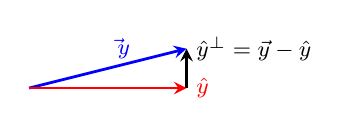
\begin{tikzpicture}[scale=0.50, baseline={([yshift={-\ht\strutbox}]current bounding box.north)}]
    \draw[line width=1pt,black,-stealth](4,0)--(4,1) node[anchor=south west]{};
    \draw[line width=1pt,blue,-stealth](0,0)--(4,1) node[anchor=south west]{};
    \draw[line width=1pt,red,-stealth](0,0)--(4,0) node[anchor=south]{}; 
    \draw [line width=0.5pt]
      (2,1) coordinate (v) node[right] {\footnotesize{$\color{blue}\vec{}{y}$}}
      (4,1) coordinate (d) node[right] {\footnotesize{$\hat{y}^\perp=\vec{y}-\hat{y}$}}
      (4,0) coordinate (u) node[right] {\footnotesize{$\color{red}\hat{y}$}};
  \end{tikzpicture}
\end{theorem}

\begin{theorem}[Best Approximation Theorem]
  Let $W$ be a subspace of $\mathbb{R}$. Let $\vec{y}\in\mathbb{R}^n$ and $\hat{y}=\text{proj}_W(\vec{}y)$. 
  Then $\hat{y}$ is closest point to $\vec{y}$ in $W$. That is $\forall\vec{v}\ne\vec{y}\;\; ||\vec{y}-\hat{y}||<||\vec{y}-\vec{v}||$  
\end{theorem}

\begin{theorem}[Orth. Proj. with Orthonormal Bases]
  Let $W$ subspace in $\mathbb{R}^n$. 
  Let $\{\vec{u}_1, ..., \vec{u}_p\}$ be an orthonormal basis of  $W$.
  $\text{proj}_W(\vec{y})=(\vec{y}\cdot\vec{u}_1)\vec{u}_1 + ... + (\vec{y}\cdot\vec{u}_p)\vec{u}_p$
  Let $U=(\vec{u}_1\; \vec{u}_2\; ...\; \vec{u}_p)$. Then $\text{proj}_W(\vec{y})=UU^T\vec{y}$
\end{theorem}

\begin{theorem}[Normal Equations and Least-Squares Sol.]
  The set of least squares solutions of $A\vec{x}=\vec{b}$ coincide the non-empty solutions of the Normal equation.
\end{theorem}

\subsection{Fact about the Orthogonal Complements}
\begin{itemize*}
  \item $\vec{0}\in W^\perp$ since $\vec{0}\cdot\vec{w}=0$
  \item If $W\in W^\perp, c\in \mathbb{R}$ then $cW\in W^\perp$
  \item If $\vec{w}_1,\vec{w}_2\in W^\perp$ so $(\vec{w}_1+\vec{w}_2)\cdot\vec{x}=\vec{w}_1\cdot\vec{x}+\vec{w}_2\cdot\vec{x}\in W$
\end{itemize*}

\subsection{Gram-Schmit Process(G-S)}
The Gram-Schmit Process is an algorithme producing an orthogonal basis.\\
Start whith $\{\vec{x}_1,...,\vec{x}_n\}$ basis for noozero subspace w of $\mathbb{R}^n$ define:\\
$\vec{v}_1=\vec{x}_1$\\
$\vec{v}_2=\vec{x}_2 -\left(\frac{\vec{x}_2\cdot\vec{v}_1}{\vec{v}_1\cdot\vec{v}_1}\right)\vec{v}_1$\\
\vdots\\
$\vec{v}_n=\vec{x}_n -\left(\frac{\vec{x}_n\cdot\vec{v}_1}{\vec{v}_1\cdot\vec{v}_1}\right)\vec{v}_1- ... -\left(\frac{\vec{x}_n\cdot\vec{v}_{n-1}}{\vec{v}_{n-1}\cdot\vec{v}_{n-1}}\right)\vec{v}_{n-1}$\\


\end{multicols}
\end{document}